%%%%%%%%%%%%%%%%%%%%%%%%%%%%%%%%%%%%%%%%%%%%%%%%%%%%%%%%%%%%%%%%%%%%
%% I, the copyright holder of this work, release this work into the
%% public domain. This applies worldwide. In some countries this may
%% not be legally possible; if so: I grant anyone the right to use
%% this work for any purpose, without any conditions, unless such
%% conditions are required by law.
%%%%%%%%%%%%%%%%%%%%%%%%%%%%%%%%%%%%%%%%%%%%%%%%%%%%%%%%%%%%%%%%%%%%



\documentclass{beamer}
\usetheme[faculty=fi]{fibeamer}
\usepackage[utf8]{inputenc}
\usepackage[
   main=english, %% By using `czech` or `slovak` as the main locale
                        %% instead of `english`, you can typeset the
                        %% presentation in either Czech or Slovak,
                        %% respectively.
   czech, slovak, greek %% The additional keys allow foreign texts to be
]{babel}            %% typeset as follows:

%%
%%    \begin{otherlanguage}{czech}    ... \end{otherlanguage}
%%    \begin{otherlanguage}{slovak}   ... \end{otherlanguage}
%%


%% These macros specify information about the presentation
\title{Sampling the flux space of microbial metabolic networks
% for (un)biased assessment of the possible functional states
} %% that will be typeset on the
\subtitle{the example of SARS-CoV-2 on the human alveolar macrophage metabolic network} %% title page.
\author{Haris Zafeiropoulos} 

%% These additional packages are used within the document:
\usepackage{ragged2e}   % `\justifying` text
\usepackage{booktabs}   % Tables
\usepackage{tabularx}
\usepackage{tikz}         % Diagrams
\usetikzlibrary{calc, shapes, backgrounds}
\usepackage{amsmath, amssymb}
\usepackage{url}          % `\url`s
\usepackage{listings}   % Code listings
\frenchspacing

\begin{document}

   \shorthandoff{-}
   \frame[c]{\maketitle}


   % Print an outline at the beginning of sections

   % 1st section using dark frames
   % \begin{darkframes}


   % SLIDE 2
   \begin{frame}{From a metabolic pathway..}
      
      \begin{tikzpicture}[overlay,remember picture]
         \node[anchor=south east,xshift=-30pt,yshift=10pt]
            at (current page.south east) {
               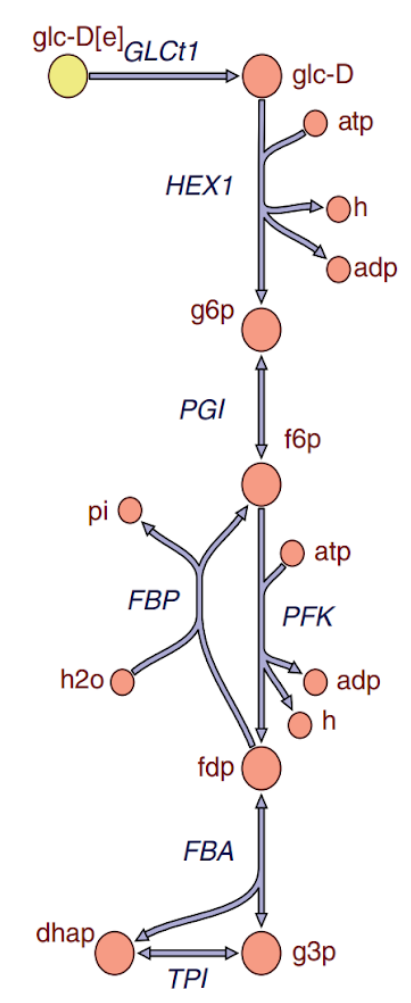
\includegraphics[width=35mm]{resources/metabolic_pathway.png}
            };
      \end{tikzpicture}

      Let us see... 

      And the mome raths outgrabe.\\\bigskip

      “Beware the Jabberwock, my son!\\
      The jaws that bite, the claws that catch!\\
      Beware the Jubjub bird, and shun\\
      The frumious Bandersnatch!”\\
   \end{frame}

   % \end{darkframes}

   
   % SLIDE 3
   \begin{frame}[label=lists]{.. to Genome-scale metabolic models}

      \begin{tikzpicture}[overlay,remember picture]
         \node[anchor=north west,xshift=30pt,yshift=-70pt]
            at (current page.north west) {
               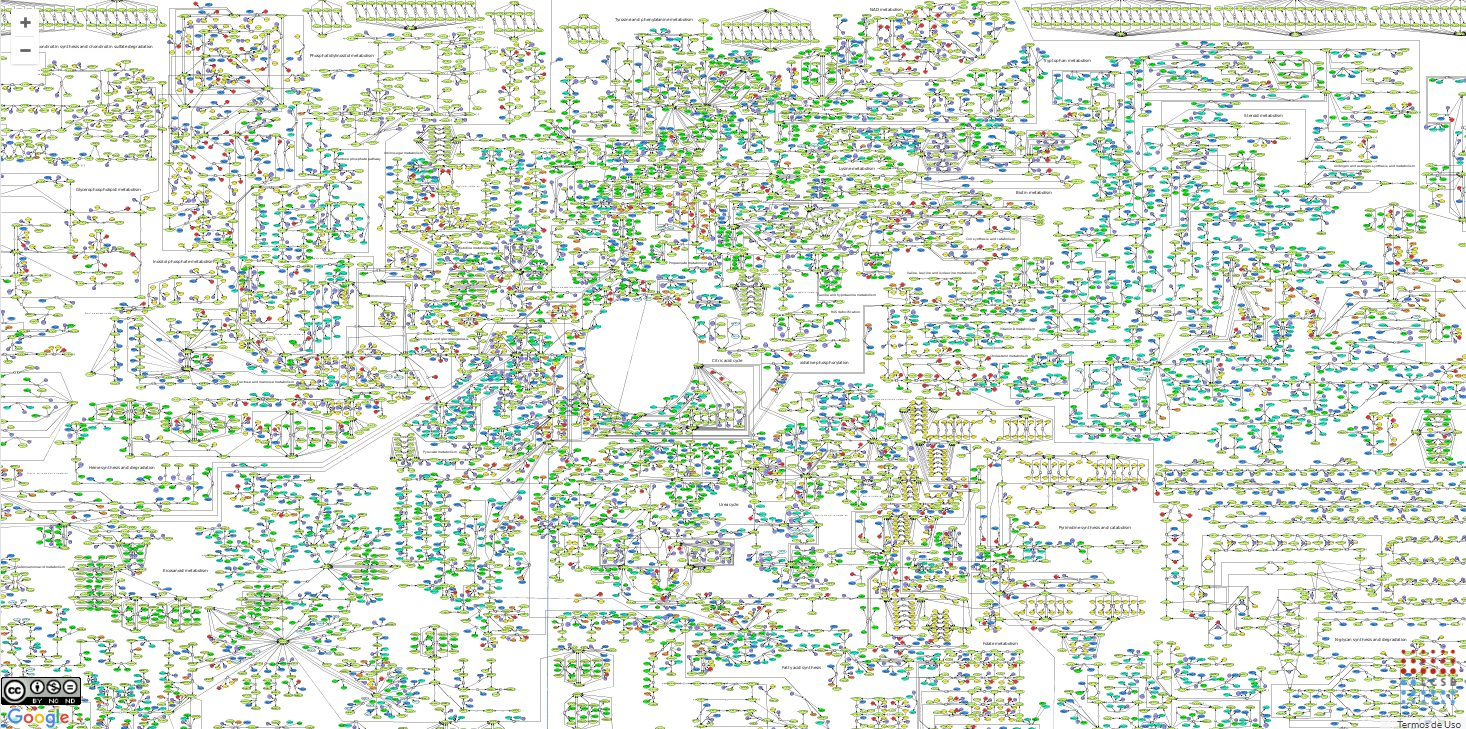
\includegraphics[width=75mm]{resources/human_network.jpg}
            };
      \end{tikzpicture}%

      Test
      \\ \bigskip
      \justifying


      The quick, brown fox jumps over a lazy
      dog. DJs flock by when MTV ax quiz prog. “Now fax quiz Jack!”

   \end{frame}


   % SLIDE 4
   \begin{frame}[label=simmonshall]{Constraint-based modeling} 

      \framesubtitle{In plain, example, and \alert{alert} flavour}
      \alert{This text} is highlighted.

      % Here is how to have a yellow box
      \begin{block}{A plain block}
            This is a plain block containing some \alert{highlighted text}.
      \end{block}
      
      % Here is how to have a grey box
      \begin{exampleblock}{An example block}
            This is an example block containing some \alert{highlighted text}.
      \end{exampleblock}

      % Here is how to have a red box
      \begin{alertblock}{An alert block}
            This is an alert block containing some \alert{highlighted text}.
      \end{alertblock} 

   \end{frame}

   % SLIDE 5 
   \begin{frame}[label=proof]{Definitions, theorems, and proofs}
      \framesubtitle{All integers divide zero}
      \begin{definition}
         $\forall a,b\in\mathds{Z}: a\mid b\iff\exists c\in\mathds{Z}:a\cdot c=b$
      \end{definition}
      \begin{theorem}
         $\forall a\in\mathds{Z}: a\mid 0$
      \end{theorem}
      \begin{proof}[Proof\nopunct]
         $\forall a\in\mathds{Z}: a\cdot 0=0$
      \end{proof}
   \end{frame}


   % SLIDE 6
   \begin{frame}[label=bibliography]{Bibliography}
      \framesubtitle{\TeX, \LaTeX, and Beamer}
      \begin{thebibliography}{9}
         \bibitem{knuth84}
               Donald~E.~Knuth.
               \emph{The \TeX book}.
               Addison-Wesley, 1984.
         \bibitem{lamport94}
               Leslie~Lamport.
               \emph{\LaTeX : A Document Preparation System}.
               Addison-Wesley, 1986.
         \bibitem{MG94}
               M.~Goossens, F.~Mittelbach, and A.~Samarin.
               \emph{The \LaTeX\ Companion}.
               Addison-Wesley, 1994.
         \bibitem{tantau04}
               Till~Tantau.
               \emph{User's Guide to the Beamer Class Version 3.01}.
               Available at \url{http://latex-beamer.sourceforge.net}.
         \bibitem{MS05}
               A.~Mertz and W.~Slough.
               Edited by B.~Beeton and K.~Berry.
               \emph{Beamer by example} In TUGboat,
                  Vol. 26, No. 1., pp. 68-73.
      \end{thebibliography}
   \end{frame}


   % Thank you SLIDE
   \begin{frame}{Thank you for your attention}
         
         GitHub repository  : \href{https://github.com/GeomScale/dingo/}{https://github.com/GeomScale/dingo/} \\ 
         \bigskip
         email    : \href{haris-zaf@hcmr.gr}{haris-zaf@hcmr.gr} \\
         Twitter  : \href{https://twitter.com/haris_zaf}{haris\_zaf} \\
         web-site : \url{https://hariszaf.github.io/} \\


         % Logos   
         % -------------- 
         % UoC
         \begin{tikzpicture}[overlay,remember picture]
            \node[anchor=south west,
                  xshift=-350pt,
                  yshift=10pt]
                  at (current page.south east) {
                     
\includegraphics[height=17mm]{
                        resources/UoC_logo.png
                     }
                  };
         \end{tikzpicture}

         % IMBBC
         \begin{tikzpicture}[overlay,remember picture]
            \node[anchor=south east,
               xshift=-185pt,
               yshift=25pt]
               at (current page.south east) {
                  
\includegraphics[width=35mm]{resources/logo-imbbc.png}
               };
         \end{tikzpicture}%

         % HCMR
         \begin{tikzpicture}[overlay,remember picture]
            \node[anchor=south east,
                  xshift=-125pt,
                  yshift=10pt]
                  at (current page.south east) {
                     
\includegraphics[height=20mm]{
                        resources/hcmr-logo.png
                     }
                  };
         \end{tikzpicture}%


         % GeomScale
         \begin{tikzpicture}[overlay,remember picture]
            \node[anchor=south east,
                  xshift=-5pt,
                  yshift=22pt]
                  at (current page.south east) {
                     
\includegraphics[width=40mm]{
                        resources/geomscale-logo.png
                     }
                  };
         \end{tikzpicture}

   \end{frame}



\end{document}
